\subsection{x86}

\subsubsection{\NonOptimizing MSVC}

Итак, компилируем:

\lstinputlisting{patterns/10_strings/1_strlen/10_1_msvc_RU.asm}

\myindex{x86!\Instructions!MOVSX}
\myindex{x86!\Instructions!TEST}
Здесь две новых инструкции: \MOVSX и \TEST.

\label{MOVSX}
О первой. \MOVSX предназначена для того, чтобы взять байт из какого-либо места в памяти и положить его, 
в нашем случае, в регистр \EDX. 
Но регистр \EDX~--- 32-битный. \MOVSX означает \IT{MOV with Sign-Extend}. 
Оставшиеся биты с 8-го по 31-й \MOVSX сделает единицей, если исходный байт в памяти имеет знак \IT{минус}, 
или заполнит нулями, если знак \IT{плюс}.

И вот зачем всё это.

По умолчанию в MSVC и GCC тип \Tchar~--- знаковый. Если у нас есть две переменные, одна \Tchar, а другая \Tint 
(\Tint тоже знаковый), и если в первой переменной лежит -2 (что кодируется как \TT{0xFE}) и мы просто 
переложим это в \Tint, 
то там будет \TT{0x000000FE}, а это, с точки зрения \Tint, даже знакового, будет 254, но никак не -2. 
-2 в переменной \Tint кодируется как \TT{0xFFFFFFFE}. Для того чтобы значение \TT{0xFE} из переменной типа 
\Tchar переложить 
в знаковый \Tint с сохранением всего, нужно узнать его знак и затем заполнить остальные биты. 
Это делает \MOVSX.

См. также об этом раздел
 \q{\IT{\SignedNumbersSectionName}}~(\myref{sec:signednumbers}).

Хотя конкретно здесь компилятору вряд ли была особая надобность хранить значение \Tchar в регистре \EDX, 
а не его восьмибитной части, скажем \DL. Но получилось, как получилось. Должно быть 
\gls{register allocator} компилятора сработал именно так.

\myindex{ARM!\Instructions!TEST}
Позже выполняется \TT{TEST EDX, EDX}. 
Об инструкции \TEST читайте в разделе о битовых полях~(\myref{sec:bitfields}).
Конкретно здесь эта инструкция просто проверяет состояние регистра \EDX на 0.

\subsubsection{\NonOptimizing GCC}

Попробуем GCC 4.4.1:

\lstinputlisting{patterns/10_strings/1_strlen/10_3_gcc.asm}

\label{movzx}
\myindex{x86!\Instructions!MOVZX}
Результат очень похож на MSVC, только здесь используется \MOVZX, а не \MOVSX. 
\MOVZX означает \IT{MOV with Zero-Extend}. Эта инструкция перекладывает какое-либо значение 
в регистр и остальные биты выставляет в 0.
Фактически, преимущество этой инструкции только в том, что она позволяет 
заменить две инструкции сразу: \TT{xor eax, eax / mov al, [...]}.

С другой стороны, нам очевидно, что здесь можно было бы написать вот так: 
\TT{mov al, byte ptr [eax] / test al, al}~--- это тоже самое, хотя старшие биты \EAX будут \q{замусорены}. 
Но будем считать, что это погрешность компилятора~--- 
он не смог сделать код более экономным или более понятным. 
Строго говоря, компилятор вообще не нацелен на то, чтобы генерировать понятный (для человека) код.

\myindex{x86!\Instructions!SETcc}
Следующая новая инструкция для нас~--- \SETNZ. В данном случае, если в \AL был не ноль, 
то \TT{test al, al} выставит флаг \ZF в 0, а \SETNZ, если \TT{ZF==0} 
(\IT{NZ} значит \IT{not zero}) выставит 1 в \AL. 
Смысл этой процедуры в том, что 
\IT{если AL не ноль, выполнить переход на} \TT{loc\_80483F0}.
Компилятор выдал немного избыточный код, но не будем забывать, что оптимизация выключена.

\subsubsection{\Optimizing MSVC}
\label{strlen_MSVC_Ox}

Теперь скомпилируем всё то же самое в MSVC 2012, но с включенной оптимизацией (\Ox):

\lstinputlisting[caption=\Optimizing MSVC 2012 /Ob0]{patterns/10_strings/1_strlen/10_2_RU.asm}

Здесь всё попроще стало. Но следует отметить, что компилятор обычно может так хорошо использовать регистры 
только на небольших функциях с небольшим количеством локальных переменных.

\myindex{x86!\Instructions!INC}
\myindex{x86!\Instructions!DEC}
\INC/\DEC --- это инструкции \glslink{increment}{инкремента}-\glslink{decrement}{декремента}. Попросту говоря~--- 
увеличить на единицу или уменьшить.

\clearpage
\subsubsectionold{\Optimizing MSVC + \olly}
\myindex{\olly}

Можем попробовать этот (соптимизированный) пример в \olly.  Вот самая первая итерация:

\begin{figure}[H]
\centering
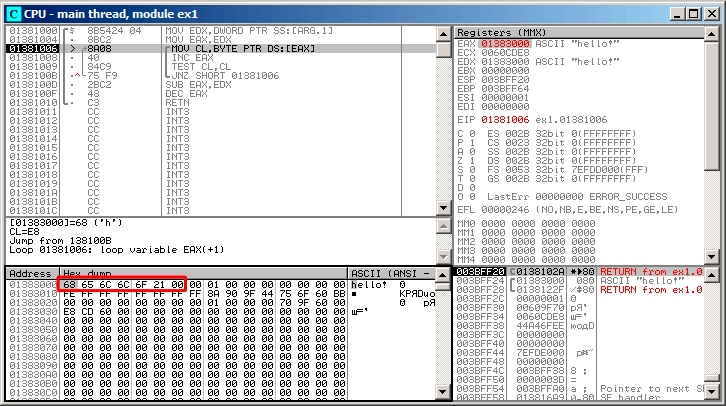
\includegraphics[scale=\FigScale]{patterns/10_strings/1_strlen/olly1.png}
\caption{\olly: начало первой итерации}
\label{fig:strlen_olly_1}
\end{figure}

Видно, что \olly обнаружил цикл и, для удобства, \IT{свернул} инструкции тела цикла в скобке.

Нажав правой кнопкой на \EAX, можно выбрать \q{Follow in Dump} 
и позиция в окне памяти будет как раз там, где надо.

Здесь мы видим в памяти строку \q{hello!}.
После неё имеется как минимум 1 нулевой байт, затем случайный мусор.
Если \olly видит, что в регистре содержится адрес какой-то строки, он показывает эту строку.

\clearpage
Нажмем F8 (\stepover) столько раз, чтобы текущий адрес снова был в начале тела цикла:

\begin{figure}[H]
\centering
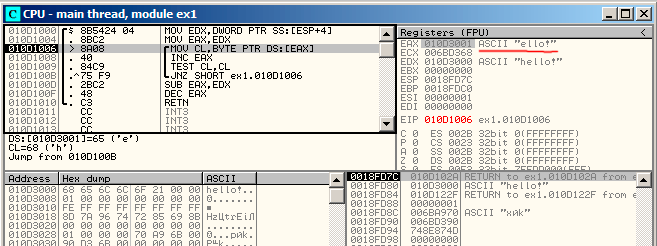
\includegraphics[scale=\FigScale]{patterns/10_strings/1_strlen/olly2.png}
\caption{\olly: начало второй итерации}
\label{fig:strlen_olly_2}
\end{figure}

Видно, что \EAX уже содержит адрес второго символа в строке.

\clearpage
Будем нажимать F8 достаточное количество раз, чтобы выйти из цикла:

\begin{figure}[H]
\centering
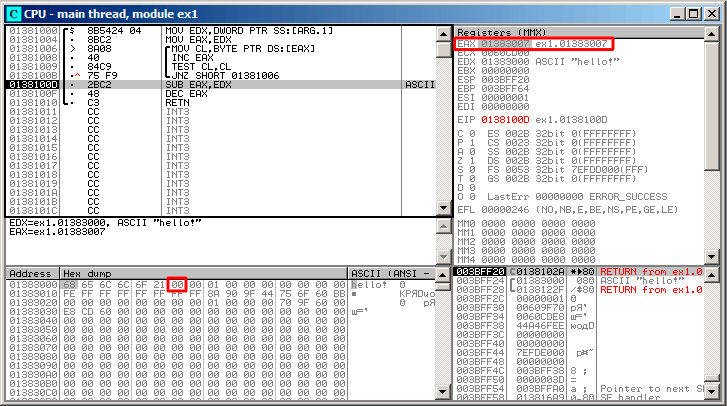
\includegraphics[scale=\FigScale]{patterns/10_strings/1_strlen/olly3.png}
\caption{\olly: сейчас будет вычисление разницы указателей}
\label{fig:strlen_olly_3}
\end{figure}

Увидим, что \EAX теперь содержит адрес нулевого байта, следующего сразу за строкой.

А \EDX так и не менялся~--- он всё ещё указывает на начало строки.
Здесь сейчас будет вычисляться разница между этими двумя адресами.

\clearpage
Инструкция \SUB исполнилась:

\begin{figure}[H]
\centering
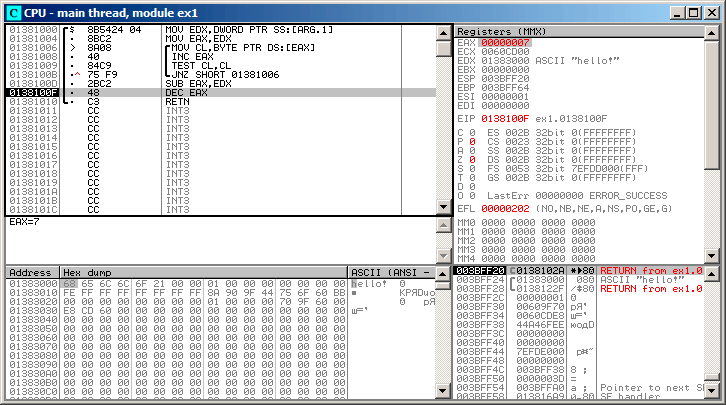
\includegraphics[scale=\FigScale]{patterns/10_strings/1_strlen/olly4.png}
\caption{\olly: сейчас будет декремент \EAX}
\label{fig:strlen_olly_4}
\end{figure}

Разница указателей сейчас в регистре \EAX~--- 7.

Действительно, длина строки \q{hello!}~--- 6, 
но вместе с нулевым байтом\EMDASH{}7.
Но \TT{strlen()} должна возвращать количество ненулевых символов в строке.
Так что сейчас будет исполняться декремент и выход из функции.



\subsubsection{\Optimizing GCC}

Попробуем GCC 4.4.1 с включенной оптимизацией (ключ \Othree):

\lstinputlisting{patterns/10_strings/1_strlen/10_3_gcc_O3.asm}

Здесь GCC не очень отстает от MSVC за исключением наличия \MOVZX. 

Впрочем, \MOVZX здесь явно можно заменить на \TT{mov dl, byte ptr [eax]}.

Но возможно, компилятору GCC просто проще помнить, что у него под переменную типа \Tchar отведен целый 
32-битный регистр \EDX и быть уверенным в том, что старшие биты регистра не будут замусорены.

\label{strlen_NOT_ADD}
\myindex{x86!\Instructions!NOT}
\myindex{x86!\Instructions!XOR}
Далее мы видим новую для нас инструкцию \NOT. Эта инструкция инвертирует все биты в операнде. 
Можно сказать, что здесь это синонимично инструкции \TT{XOR ECX, 0ffffffffh}. 
\NOT и следующая за ней инструкция \ADD вычисляют разницу указателей и отнимают от результата единицу. 
Только происходит это слегка по-другому. Сначала \ECX, где хранится указатель на \IT{str}, 
инвертируется и от него отнимается единица.
См. также раздел: \q{\SignedNumbersSectionName}~(\myref{sec:signednumbers}).

Иными словами, в конце функции, после цикла, происходит примерно следующее: 

\begin{lstlisting}
ecx=str;
eax=eos;
ecx=(-ecx)-1; 
eax=eax+ecx
return eax
\end{lstlisting}

\dots~что эквивалентно:

\begin{lstlisting}
ecx=str;
eax=eos;
eax=eax-ecx;
eax=eax-1;
return eax
\end{lstlisting}

Но почему GCC решил, что так будет лучше? Трудно угадать.
Но наверное, оба эти варианта работают примерно одинаково в плане эффективности и скорости.
